% Chapter Template

\chapter{Evaluation of Results and Discussion} % Main chapter title

\label{Chapter5} % Change X to a consecutive number; for referencing this chapter elsewhere, use \ref{ChapterX}

\lhead{Chapter 5. \emph{Evaluation of Results and Discussion}} % Change X to a consecutive number; this is for the header on each page - perhaps a shortened title

This chapter discusses the ability of an implementation of defeasible reasoning to model a construct in comparison with machine learning. The chapter presents and discusses the results of the experiment performed in the previous chapter. A comparative analysis of both techniques is performed using the evaluation techniques gathered literature review.

\section{Results}

% dat = read.csv("alldataallresults.csv", header = TRUE)
% threshold <- 0
% subset(dat, dat["time"] < threshold)
% colnames(dat[5:37])
% cor(dat[4:37])
% cor(dat[,c(5,7,9,10,34,36,40,42)])

The research question posed at the start of this project is focused on the ability of two techniques to represent and predict the value of a construct. In order to determine the ability of the techniques to measure the construct the concurrent and convergent validity of the results is determined.

\subsection{Predictive Capacity}

\begin{table}[!htbp]
\centering
\begin{tabular}{|c|c|c|c|}
\hline
                                &  10-fold & 20-fold & 40-fold \\ \hline
Additive Regression             & 85.8072  & 83.5995  & 82.0641 \\
ANN                             & 137.238 & 126.9808 & 141.3834 \\
Regression                      & 80.8231 & 80.9963 & 80.2697 \\
K Star                          & 93.6672 & 92.1658 & 91.1066 \\
Expert (Grounded Extension)     & 80.6007 & 80.5986 & 80.5241 \\
Expert (Prefered Extension)     & 80.4185 & 80.4475 &  80.3192 \\
Non-Expert (Grounded Extension) & 81.5565 & 81.6743 & 81.7295 \\
Non-Expert (Prefered Extension) & 81.5565 & 81.6743 & 81.7295 \\
\hline
\end{tabular}
\caption{Mean Absolute Error}
\label{tab:time_predictions}
\end{table}

\begin{table}[!htbp]
\centering
\begin{tabular}{|c|c|c|c|}
\hline
                                & 30\% Split  & 50\% Split  & 70\% Split \\ \hline
Additive Regression             & 93.3442  & 81.2395  & 87.8533 \\
ANN                             & 163.7684 & 152.5288 & 147.3721 \\
Regression                      & 83.1717 & 80.868 & 83.589 \\
K Star                          & 101.9482 & 93.8966 & 92.0756 \\
Expert (Grounded Extension)     & 81.0625 & 78.0558 & 78.7381 \\
Expert (Prefered Extension)     & 80.4185 & 80.4475 &  80.3192 \\
Non-Expert (Grounded Extension) & 79.5426 & 77.2909 & 79.9484 \\
Non-Expert (Prefered Extension) & 79.5426 & 77.2909 & 79.9484 \\
\hline
\end{tabular}
\caption{Expert knowledge base concurrent validity against time}
\label{tab:time_predictions}
\end{table}



\subsection{Concurrent Validity (Construct)}

The concurrent validity of the defeasible constructs was measured by performing regressions against time (tables ~\ref{tab:eccurrent_time} and ~\ref{tab:neccurrent_time}). Time is an objective performance measure that is similar to MWL. For all knowledge bases the error rate is high. The error rate for the expert knowledge base is slightly lower than the non-expert knowledge base. As the values of time can be anywhere from 0 to a few hundred seconds predicting time exactly from the values of MWL is extremely error prone. Moreover, the precision required for the construct of MWL doesn't need to be as precise as seconds. Correlation provides a better understanding of the performance of the knowledge base in this case. The results show a much stronger correlation between the knowledge base of the expert and time than the knowledge base of the non-expert. This provides some confirmation that the implementation is modeling defeasible knowledge bases correctly as it is expected that the knowledge base of the expert should more accurately represent MWL that that of the non-expert. The preferred extension of the knowledge base of the expert performed better than the grounded extension. The preferred extension and the grounded extension of the non-expert were determined to be equivalent by the software and so show the same results.

\begin{table}[!htbp]
\centering
\begin{tabular}{|c|c|c|}
\hline
                            &  expertGrounded & expertPref \\ \hline
Correlation coefficient     & 0.3362        & 0.3414      \\
Mean absolute error         & 80.6007       & 80.4185     \\
Root mean squared error     & 110.3579      & 110.1416  \\
Relative absolute error     & 95.9998\%     & 95.7829\% \\
Root relative squared error & 94.0706\%     & 93.8863\% \\
\hline
\end{tabular}
\caption{Expert knowledge base concurrent validity against time}
\label{tab:eccurrent_time}
\end{table}

\begin{table}[!htbp]
\centering
\begin{tabular}{|c|c|c|}
\hline
                            &   non-expertGrounded  & non-expertPref \\ \hline
Correlation coefficient     &  0.2046         & 0.2046  \\
Mean absolute error         &  81.5565        & 81.5565  \\
Root mean squared error     & 114.6813       & 114.6813  \\
Relative absolute error     & 97.1383\%      & 97.1383\%  \\
Root relative squared error & 97.756\%       & 97.756\%  \\
\hline
\end{tabular}
\caption{Non-Expert knowledge base concurrent validity against time}
\label{tab:neccurrent_time}
\end{table}

The performance of the machine learning algorithms vary dramatically (table ~\ref{tab:ml1currenttime} and ~\ref{tab:ml2currenttime}). It is interesting to note that simple linear regression using one variable doesn't out perform the regression based on the non-expert knowledge base. Decision table, kstar and additive regression have error rates higher than the expert knowledge base. Decision table and kstar don't correlate well with time although additive regression performs nearly as well as the expert knowledge base. A linear regression outperforms all of the techniques and can predict task time with the strongest correlation.

\begin{table}[!htbp]
\centering
\begin{tabular}{|c|c|c|}
\hline
                            & Simple Linear Regression   & decisionTable\\ \hline
Correlation coefficient     & 0.1783        & 0.2788    \\
Mean absolute error         & 84.839        & 83.8164   \\
Root mean squared error     & 115.9599      & 115.7615  \\
Relative absolute error     & 101.0479\%    & 99.83\%   \\
Root relative squared error & 98.8458\%     & 98.6767\% \\
\hline
\end{tabular}
\caption{Simple Linear Regression and Decision Table concurrent validity against time}
\label{tab:ml1currenttime}
\end{table}

\begin{table}[!htbp]
\centering
\begin{tabular}{|c|c|c|c|}
\hline
                            & kstar & additiveregression & Linear Regression\\ \hline
Correlation coefficient     &  0.2428       & 0.3358    & 0.4201 \\
Mean absolute error         &  93.6672      & 85.8072   & 80.8231 \\
Root mean squared error     &  130.8713     & 116.8993  & 107.0807  \\
Relative absolute error     & 111.5627\%   & 102.201 \% & 96.2647\%\\
Root relative squared error &  111.5565\%   & 99.6466\%  & 91.2771\%\\
\hline
\end{tabular}
\caption{K Star, Additive Regression and Linear Regression concurrent validity against time}
\label{tab:ml2currenttime}
\end{table}

The second test of concurrent validity was performed using task membership. Again it is seen that the knowledge base of the expert out performs that of the non-expert. Neither knowledge base can predict task membership as well as the machine learning classifiers (table ~\cite{tab:ecurrenttask} and ~\cite{tab:necurrenttask}). %why?

\begin{table}[!htbp]
\centering
\begin{tabular}{|c|c|c|}
\hline
                                 & expertGrounded  & expertPref \\ \hline
Correctly Classified Instances   & 8.8319\%      & 9.4017\% \\
Incorrectly Classified Instances & 91.1681\%     & 90.5983\% \\
Kappa statistic                  & 0.034         & 0.0401    \\
Mean absolute error              & 0.0856        & 0.0856    \\
Root mean squared error          & 0.2069        & 0.2069    \\
Relative absolute error          & 98.9565\%     & 98.9251\% \\
Root relative squared error      & 99.478\%      & 99.4743\% \\
\hline
\end{tabular}
\caption{Expert knowledge base concurrent validity against task membership}
\label{tab:ecurrenttask}
\end{table}

\begin{table}[!htbp]
\centering
\begin{tabular}{|c|c|c|}
\hline
                                 & non-expertGrounded  & non-expertPref \\ \hline
Correctly Classified Instances   & 7.4074\%         & 7.4074\%  \\
Incorrectly Classified Instances & 92.5926\%        & 92.5926\%  \\
Kappa statistic                  & 0.0206           & 0.0206  \\
Mean absolute error              & 0.086            & 0.086   \\
Root mean squared error          & 0.2075           & 0.2075  \\
Relative absolute error          & 99.4773\%       & 99.4773\%  \\
Root relative squared error      & 99.7922\%       & 99.7922\%  \\
\hline
\end{tabular}
\caption{Non-Expert knowledge base concurrent validity against task membership}
\label{tab:necurrenttask}
\end{table}

The results of the machine learning classifiers show that Naive Bayes performs best out of the group, closely followed by logistic regression (table ~\ref{tab:ml1currenttask} and ~\ref{tab:ml2currenttask}). 

\begin{table}[!htbp]
\centering
\begin{tabular}{|c|c|c|c|}
\hline
                                 & Bayes Net  & Decision Table  & Logistic Regression \\ \hline
Correctly Classified Instances   & 11.3636\%      & 11.8182\%  & 23.6364\%  \\
Incorrectly Classified Instances & 88.6364\%      & 88.1818\% & 76.3636\%   \\
Kappa statistic                  & 0.0714         & 0.0762    & 0.2         \\
Mean absolute error              & 0.083          & 0.0838    & 0.0709      \\
Root mean squared error          & 0.2041         & 0.2042    & 0.22        \\
Relative absolute error          & 95.6447\%      & 96.5821\% & 81.6907\%   \\
Root relative squared error      & 97.9663\%      & 98.0531\% & 105.6358\%  \\
\hline
\end{tabular}
\caption{Bayes Net, Decision Table and Logistic Regression concurrent validity against task membership}
\label{tab:ml1currenttask}
\end{table}


\begin{table}[!htbp]
\centering
\begin{tabular}{|c|c|c|}
\hline
                                 & Naive Bayes & Random Tree\\ \hline
Correctly Classified Instances   & 25\%      &  14.7727\%\\
Incorrectly Classified Instances & 75\%      &  85.2273\%\\
Kappa statistic                  & 0.2143    & 0.1071\\
Mean absolute error              & 0.07      & 0.0775\\
Root mean squared error          & 0.2262    & 0.2784\\
Relative absolute error          & 80.6802\% & 89.2857\%\\
Root relative squared error      & 108.5826\% & 133.6306\%\\
\hline
\end{tabular}
\caption{Naive Bayes and Random Tree concurrent validity against task membership}
\label{tab:ml2currenttask}
\end{table}

It is interesting that the machine learning approach was more effective in determining task membership than the defeasible reasoning approach. This could be because the tasks don't vary MWL strongly enough. Whether this is true or not could be determined by taking some measure of the convergent validity of MWL and task number. Unfortunately this is not possible via a simple correlation. Another possibility is that the knowledge bases are failing to take into account some aspect of mental workload that could determine task membership better.

\subsection{Convergent Validity (Construct)}

In order to determine how well the constructs actually modeled MWL the convergent validity of these measures was determined. The convergent validity was determined by computing the correlation of each measure with existing measures of MWL. 

It can be seen that the expert's knowledge base correlates strongly with the other measures for MWL (table ~\ref{tab:corrmwlone}, ~\ref{tab:corrmwltwo} and ~\ref{tab:corrmwlthree}). There is a moderate correlation between other measures of MWL and and the non-expert's knowledge base. 

Time does not correlate well with existing measures of MWL. This underlines one of the shortcomings of the machine learning approach for modeling constructs. A value must already exist in the data set that has a strong convergent validity with the construct being modeled. It was possible to predict task time most accurately using linear regression, however, this prediction is not useful to an expert if it doesn't have a high convergent validity with MWL. The only way to predict the value for a construct using machine learning is to have an expert label the data by hand. Labeling this data is a time consuming process as it will have to be done for very large data sets in order for the model to be trained accurately. As this work is tedious it may be difficult to guarantee that the expert has devoted equal attention to labeling all instances accurately. Moreover, the time that the expert spends labeling the data is taken away from their real work which may make many experts hesitant to get involved with such projects.

\begin{table}[!htbp]
\centering
\begin{tabular}{|c|c|c|c|}
\hline
                 &  time     & NASA      &  WP        \\ \hline
time             & 1.0000000 & 0.2174278 & 0.2036869  \\
NASA             & 0.2174278 & 1.0000000 & 0.5836784 \\
WP               & 0.2036869 & 0.5836784 & 1.0000000 \\
expertGroundedExt  & 0.2928288 & 0.7233711 & 0.8593995 \\
expertPref1        & 0.2882237 & 0.7247067 & 0.8499664 \\
non-expertGroundedExt & 0.1245360 & 0.5518035 & 0.5648483 \\
non-expertPref1       & 0.1245360 & 0.5518035 & 0.5648483 \\
\hline
\end{tabular}
\caption{Pearson correlation of measures of MWL (1)}
\label{tab:corrmwlone}
\end{table}

\begin{table}[!htbp]
\centering
\begin{tabular}{|c|c|c|}
\hline
                 & expertGroundedExt & expertPref1 \\ \hline
time             & 0.2928288 & 0.2882237        \\
NASA             & 0.7233711 & 0.7247067        \\
WP               & 0.8593995 & 0.8499664        \\
expertGroundedExt  & 1.0000000 & 0.9860579         \\
expertPref1        & 0.9860579 & 1.0000000        \\
non-expertGroundedExt & 0.6243195 & 0.6304207        \\
non-expertPref1       & 0.6243195 & 0.6304207        \\
\hline
\end{tabular}
\caption{Pearson correlation of measures of MWL (2)}
\label{tab:corrmwltwo}
\end{table}

\begin{table}[!htbp]
\centering
\begin{tabular}{|c|c|c|}
\hline
                 & non-expertGroundedExt & non-expertPref1 \\ \hline
time                & 0.1245360  & 0.1245360 \\
NASA                & 0.5518035  & 0.5518035 \\
WP                  & 0.5648483  & 0.5648483 \\
expertGroundedExt   & 0.6243195  & 0.6243195 \\
expertPref1         & 0.6304207  & 0.6304207 \\
non-expertGroundedExt & 1.0000000  & 1.0000000 \\
non-expertPref1       & 1.0000000  & 1.0000000 \\
\hline
\end{tabular}
\caption{Pearson correlation of measures of MWL (3)}
\label{tab:corrmwlthree}
\end{table}

One situation in which this approach might be advantageous is to use the defeasible reasoning system to `label' the data instead of an expert having to endure the labour of labeling the data by hand. The implementation can be used to elicit a knowledge base from the expert and then run on training data applying labels to each row. Machine learning can then be used to determine the values for a construct in future instances of the data. This hybrid approach offers the best of both worlds as the expert can still obtain feedback about his knowledge base while the implementation can benefit from the speed and automatic computation of machine learning. Tables ~\ref{tab:mlhybrid1} and ~\ref{tab:mlhybrid2} show that ML can predict values for MWL well when provided with a labeled training set of data.

\begin{table}[!htbp]
\centering
\begin{tabular}{|c|c|c|c|}
\hline
                            & Simple Linear Regression   & decisionTable  & kstar\\ \hline
Correlation coefficient     & 0.6508        & 0.5861         & 0.2428       \\
Mean absolute error         & 9.991        & 10.7846        & 93.6672       \\
Root mean squared error     & 12.4932      & 13.6643       & 130.8713       \\
Relative absolute error     & 73.8692\%    & 79.7374\%        & 111.5627\%  \\
Root relative squared error & 75.8265\%     & 82.9345\%      & 111.5565\%   \\
\hline
\end{tabular}
\caption{Error and correlation results for prediciting MWL values according to expert's prefered extension (1)}
\label{tab:mlhybrid1}
\end{table}


\begin{table}[!htbp]
\centering
\begin{tabular}{|c|c|c|}
\hline
                            & additiveregression & Linear Regression\\ \hline
Correlation coefficient     & 0.8447    & 0.9392 \\
Mean absolute error         & 7.446      & 3.8686 \\
Root mean squared error     & 9.5961    & 5.6552  \\
Relative absolute error     & 55.0526\% & 28.6028\%\\
Root relative squared error & 58.2429\%  & 34.3239\%\\
\hline
\end{tabular}
\caption{Error and correlation results for predicting MWL values according to expert's prefered extension (2)}
\label{tab:mlhybrid2}
\end{table}


\begin{figure}
\centering
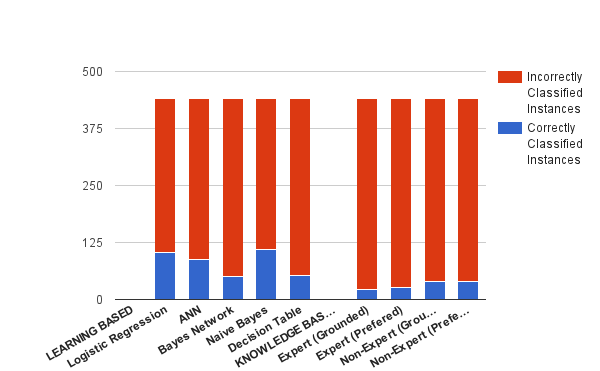
\includegraphics[width=\linewidth]{mae_time}
\caption{Caption}
\label{fig:my_label}
\end{figure}


\begin{figure}
\centering
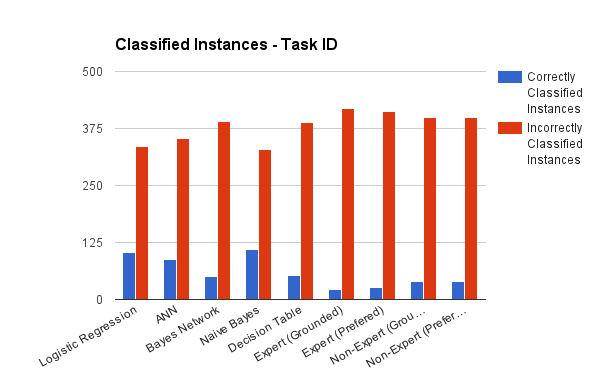
\includegraphics[width=\linewidth]{classified_instances}
\caption{Caption}
\label{fig:my_label}
\end{figure}

\section{Summary and Final Recommendations}

This chapter presented the results obtained in the experiment. Overall it is seen that linear regression performed best when presented with a prediction problem, however, it is limited to predicting features already present in the training data. This is a strong limitation of machine learning generally. In the case of MWL the value for time was chosen to represent the construct, however this was shown to have poor convergent validity with other measures of mental workload. The values for MWL developed from the experts knowledge base were found to have a strong convergent validity with another measure for MWL, NASA-TLX. It was noted that the DR implementation performed slowly and measures that could be taken in future implementations were described. Finally it was noted that the DR system could be used to label a training set used in machine learning in a hybrid approach. 